\chapter{Functional system overview}
This chapter gives a system overview on a functional level by describing the drivers, the approach of the project, the business model, high-level requirements, and the business and system use cases.
\section{Drivers}
\label{sec:drivers}
Some parameters that influence the outcome of \ac{MPI}, are:

\begin{tabular}{llll}
 	\multicolumn{1}{c}{\textbf{Tracer}} & \multicolumn{1}{c}{\textbf{Patient}} & \multicolumn{1}{c}{\textbf{Technology}} & \multicolumn{1}{c}{\textbf{Software}} \\
		- Activity, & - Breathing artefacts, & - Modality, & - Package, \\
		- Volume, & - Cardiac motion, &  - Spatial resolution, & - Mathematical model, \\
		- Molecule size, & - BMI. & - Temporal resolution. & - Filters,\\
		- Injection speed.  & & & \makecell[l]{- \acs{ROI}.}\\
\end{tabular}

The strength of a phantom is its reproducibility. Varying specific parameters provides insight into dependent and independent factor and its effect on the outcome.

Current phantoms either require modifications to clinical software packages or do not model defects in a physiological way, typically by reducing the flow through the myocardium by reducing the pump rate. This effectively ignores the complex relation between stenotic and non-stenotic arteries. Therefore, a myocardial perfusion phantom is needed that is compatible with clinical software and is able to mimic cardiac defects in a physiological way. This will increase the similarity with patient studies resulting in more reliable validation.

In addition to validation of scanners and/or software packages, the phantom can be used for education and training, to demonstrate the impact of the different parameters, but also for optimisation, of protocol and/or work flow. 

\section{Approach}
The project development cycle is defined by the V-Model. The project plan defined several research questions, in which this section answers the research questions for the first two phases: the "concept of operations" phase and "requirements and architecture" phase.

\subsection{Concept of operations}
\label{sec:concept_oper}
\subsection*{Is the D-SPECT's dynamic scanning, in comparison with other modalities (CT, MRI, PET, or SPECT), suitable for quantitative myocardial perfusion imaging?}
Quantitative flow measurements is made possible as a result of dynamic scanning.The technique is not new, \ac{CT} utilises it in past research. The solid-state detectors (Cadmium-Zinc Telluride) made dynamic scanning possible for \ac{SPECT}. The D-SPECT is a highly specialised cardiac system and is relatively new in the Netherlands. It has been employed in Japan, Canada, France, and Great-Britain. The relatively small patient population, in the Netherlands, forces clinics to choose less specialised systems in order to prevent excessive costs. However, despite its specialisation, the D-SPECT offers a very patient friendly experience due to its open design. Competitors, for example GE, use a gantry design which encloses the patient and can result in anxiety and stress.

\ac{CT} is a well established modality with the highest spatial resolution. However, its largest drawback is the direct, proportional, relation between radiation dose and the number of images taken, thereby increasing the likelihood of radiation based complication. \ac{MRI} does not rely on ionising radiation, but its lower temporal resolution makes it less suitable for dynamic imaging. It does offer the best tissue discrimination. \ac{SPECT} and \ac{PET} both use radioactive tracers to image blood flow, thus exposing the patient to some degree of radiation. However, it is not directly proportional to the number of images taken. D-SPECT offers significant dose reduction, due to more sensitive detectors, which reduces the strain and risk for patients.

In addition, traditional \ac{SPECT} is, on average, 22\% less expensive than the current gold standard, \ac{PET} in cardiac imaging. D-SPECT is supposed to be even less expensive and faster with better image resolution. 

In summary, although the D-SPECT is relatively new in the Netherlands, it is more widely employed in Japan, Canada, France, and Great-Britain. The highly cardiac specialised system, its patient friendly design, the ability to scan faster and more accurate at significant dose reductions, make the D-SPECT suitable for quantitative myocardial perfusion imaging. 

\subsection{What must the myocardial perfusion phantom be able to simulate to validate quantitative MPI?}
\label{sec:what_perf}
The phantom must be compatible with clinical practice, i.e. use clinical protocols and hard-/software. Patients are scanned in a D-SPECT scanner while lying down, face up (supine). The scans are evaluated using 4DM software. 

The phantom must be suitable for an \ac{AIF} ROI in the left atrium. Alternatively, in case of poor results, the ROI can be reshaped and placed in the left ventricle. The software determines the perfusion in 17 areas of the left ventricle's myocardium, at a basal, mid and apical level, and at the apex. These segments are supplied via branches of the three coronary arteries, i.e. the RCA, LAD, and LCx. 4DM calculates individual flow rates for each segment. Therefore, the phantom should contain 17 segments where each segment is either static or with variable flow that can be measured. 

A single flow source is to be used that supplies the RCA, LAD, and LCx. From an anatomical viewpoint, the coronary arteries are supplied from the aorta. The phantom could mimic this anatomical structure, which is impractical. Instead, it is possible to supply the coronary arteries from a dedicated flow source significantly decreasing the total volume of liquid being displaced. Care must be taken such that the ratio of contrast remains equivalent. Since the entire myocardium is supplied by three coronary arteries, stenosis in one of the arteries, or its branches, results in different flow behaviour which cannot be mimicked by reducing the overall flow to the myocardium alone.

Every tracer behaves differently. For D-SPECT, Technetium (\textsuperscript{99m}Tc) Tetrofosmin is used. Only a small part of the total activity is absorbed by the myocardium; approximately 1.2\% in 5 minutes. Therefore, the uptake of tracer into tissue is not a necessity, it will be a design choice. 

\section{Business model}
\label{sec:bus_model}
Dynamic scanning yield quantitative results, i.e. absolute perfusion rates, which require proper validation. Phantom studies are, to a high degree, suitable for such purpose. An added benefit of these studies, is that it provides insight into the effect of different parameters on the outcome, which in turn impacts patient treatment. These insights can be used for calibration or optimisation, e.g. tracer protocol or work flow. Some examples would be determining optimal (patient dependable) activity or injection speed, or placement of the placement of peripherals.

In short, the phantom can be used for validation, education, training, calibration or optimisation. 

The phantom will distinguish itself from other phantoms due to its more true-to-nature design, ability to physiologically mimic cardiac defects, and the possibility of modelling different compartment models.

The primary focus remains on the current application of \ac{MPI} as performed at the ZGT in Hengelo, Overijssel.

Please note, the phantom is developed during a master thesis to support the research of a PhD thesis. Therefore, there is no business plan to ensure profit, and to payback investments.

\section{Requirements}
\rrod{Verify the AIF requirements.}
This section defines the functional requirements. These are high-level requirements and are shown in table \ref{tab:funcreq}.

\begin{table}[h]
\caption{Functional requirements}
\label{tab:funcreq}
\begin{tabular}{l|p{120mm}|}
	\makecell[l]{Requirement \\ number} & \multicolumn{1}{c}{Description}\\
	\hline
	FR01 & The phantom must be able to simulate blood flow at high flow rates (aortic flow). \\ 
	\rowcolor{Gray}
	FR02 & The phantom must be able to simulate blood flow at low flow rates (myocardial flow). \\
	FR03* & An \ac{AIF} can be extracted from the left atrium, or alternatively from the left ventricle. \\
	\rowcolor{Gray}
	FR04 & Cardiac defects must simulate the complex relation between stenotic and non-stenotic arteries. \\
	FR05 & The phantom must be able to visualise (and measure) at least two active segments of the 17-segment ventricle model. \\
	\rowcolor{Gray}
	\sout{FR06} & \sout{The phantom must use a 2-compartment model (simulating contrast uptake in tissue).} \\
	FR07 & Tracer protocol must be equivalent to that used in clinical scans with D-SPECT. \\
	\rowcolor{Gray}
	\sout{FR08} & \sout{Contrast should be mixed equivalently to contrast mixing in patients.} \\
	\cline{2-2}
\end{tabular}
\raggedright
\textit{* Depending on the flexibility of the clinical software.}
\end{table}

\section{Business and system use cases}	
The myocardial perfusion phantom is used by researchers with varying goals. Primarily, the phantom set-up is a tool to validate perfusion imaging hard- and software and to educate on independent and dependent factors, see section \ref{sec:drivers}. The researcher should be able to adjust the blood flow, both in the myocardium and in the aorta, and be able to set a cardiac defect.

Please note, setting the imaging and contrast parameters are not part of the phantom itself. 
\begin{figure}[!h]
	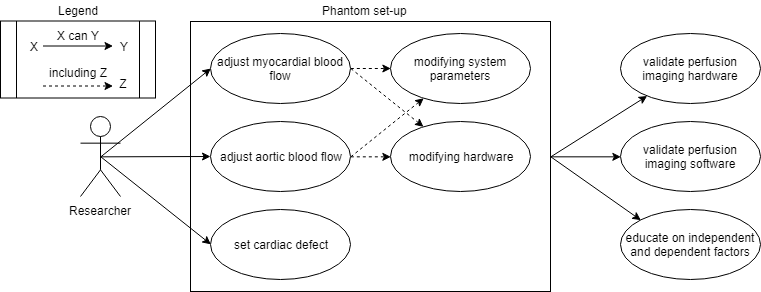
\includegraphics[width=\textwidth]{./images/usecase_diagram.png}
	\caption{Use case diagram for the prototype myocardial perfusion phantom}
	\label{fig:usecase}
\end{figure}

\section{Architectural overview}
A schematic overview of the flow set-up is shown in figure \ref{fig:funcarch}. The set-up consists of a flow generating system, e.g. mechanical pumps or pressure based, to generate the required aortic and myocardial flow, measuring systems, e.g. flow and pressure sensors, and the phantom itself, simulating the heart. The flow is controlled by means of a control system, over which the user has control. The flow parameters, i.e. flow and pressure, are measured by sensors which are monitored by a monitoring system. The monitoring system and control system cooperate such that user parameters are maintained. Figure \ref{fig:funcarch} shows a distinction between high and low flow, which is not a requirement. Low flow can be created by means of pressure difference in high and low flow circuit; increasing pressure in low flow circuit results in less volume passing through.
\begin{figure}
	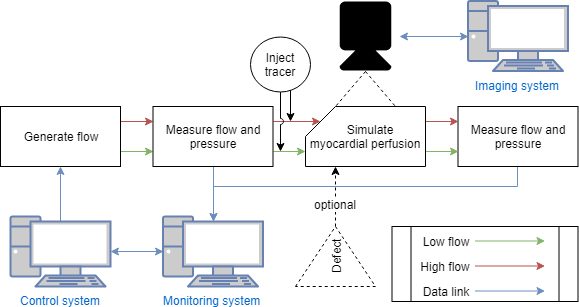
\includegraphics[width=0.75\textwidth]{./images/functional_architecture.png}
	\caption{Functional architecture for the myocardial perfusion set-up. The myocardial perfusion is simulated in normal situations and in defect situations. The manner in which a defect situation is simulated, is a design choice. \textbf{Figure for indicative purposes, subject to change}.}
	\label{fig:funcarch}
\end{figure}
